% Chapter Template
\chapter{Ensayos y Resultados} % Main chapter title
En este capítulo se expone cuales fueron las pruebas realizadas para determinar que el sistema funciona en forma correcta.
\label{Chapter4} % Change X to a consecutive number; for referencing this chapter elsewhere, use \ref{ChapterX}

\section{Banco de pruebas}
Para simular el comportamiento de un sensor de temperatura y la descarga de una batería, se implementó la placa que fue presentada en la sección \ref{hw_placa}, que para facilidad del lector se vuelve a mostrar en la figura \ref{fig:placa_básica}. 
Esta consta de dos potenciómetros que permiten simular la variación de la temperatura y la carga de la batería. Sobre la placa se conecto un conversor RS232 a TTL, para lograr la integración con el módem.

\begin{figure}[h]
  \centering
  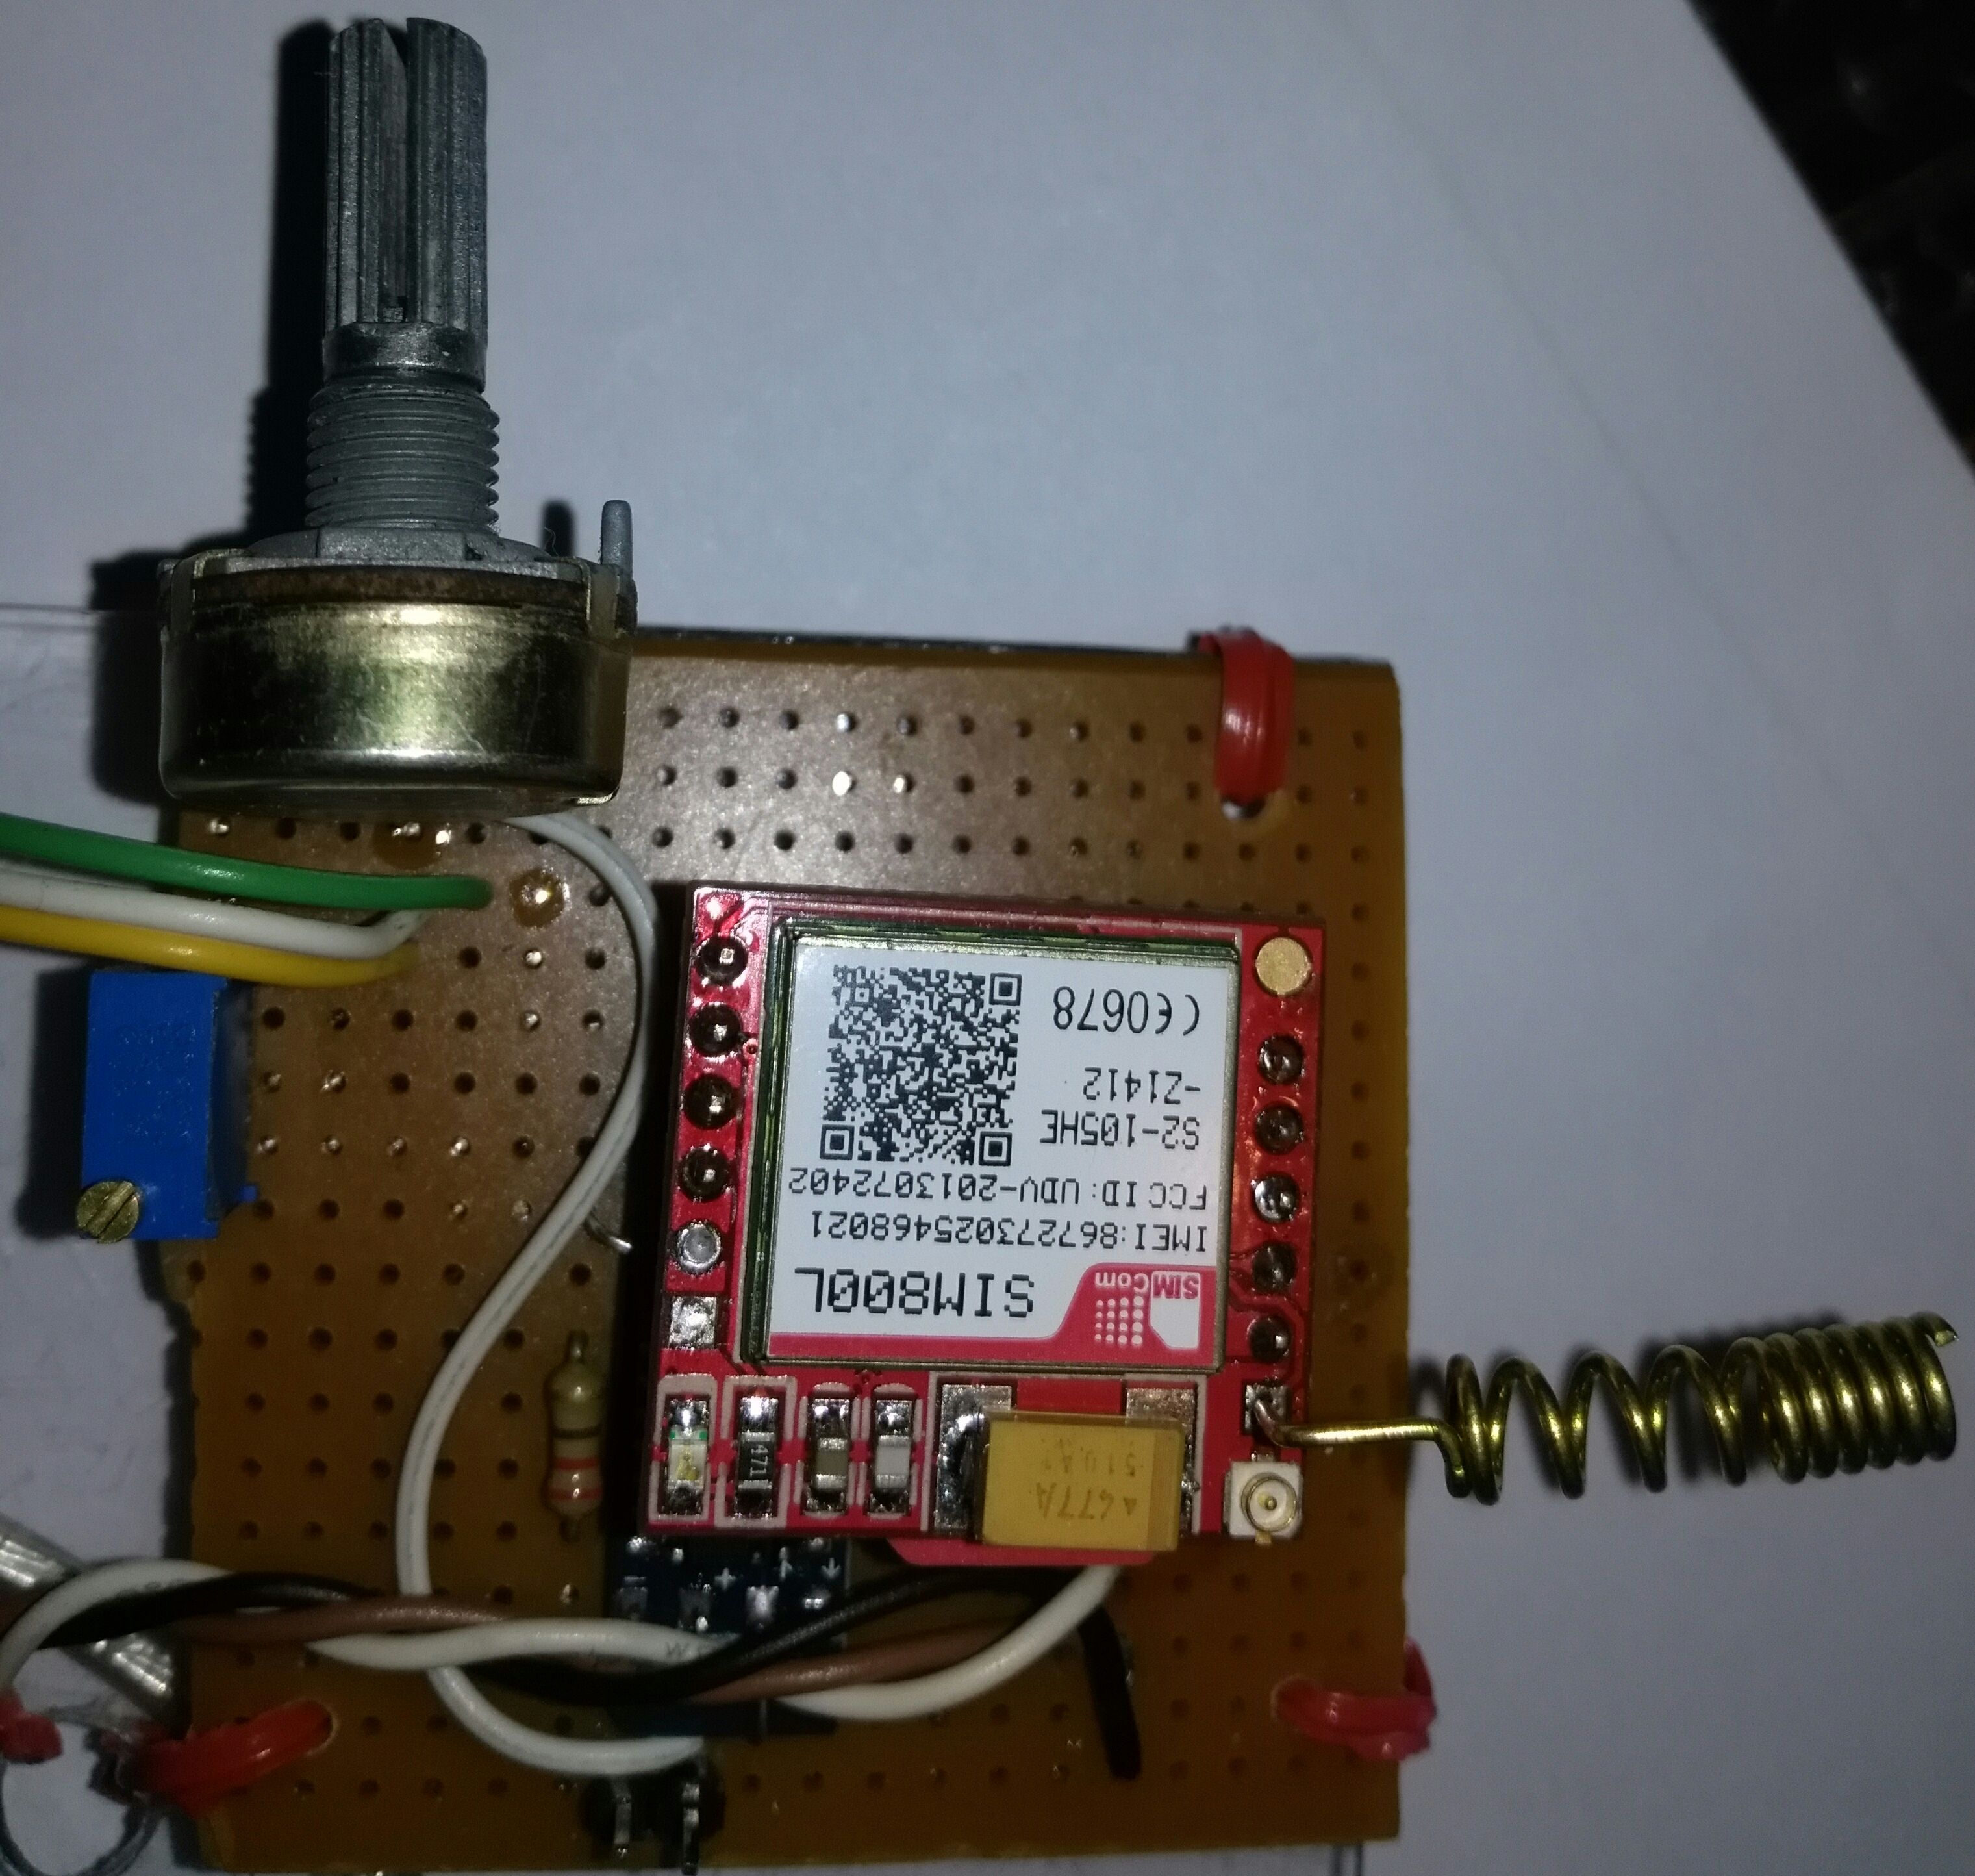
\includegraphics[scale=.1]{./Figures/placa_basica.jpg}
  \caption{Placa de simulación de temperatura y estado de la batería con el modulo SIM800l integrado.}
  \label{fig:placa_básica}
\end{figure}

En la figura \ref{fig:prototipo} se muestra la placa que contiene el módem y los componentes de simulación conectada a la CIAA-NXP. 

\begin{figure}[h]
  \centering
  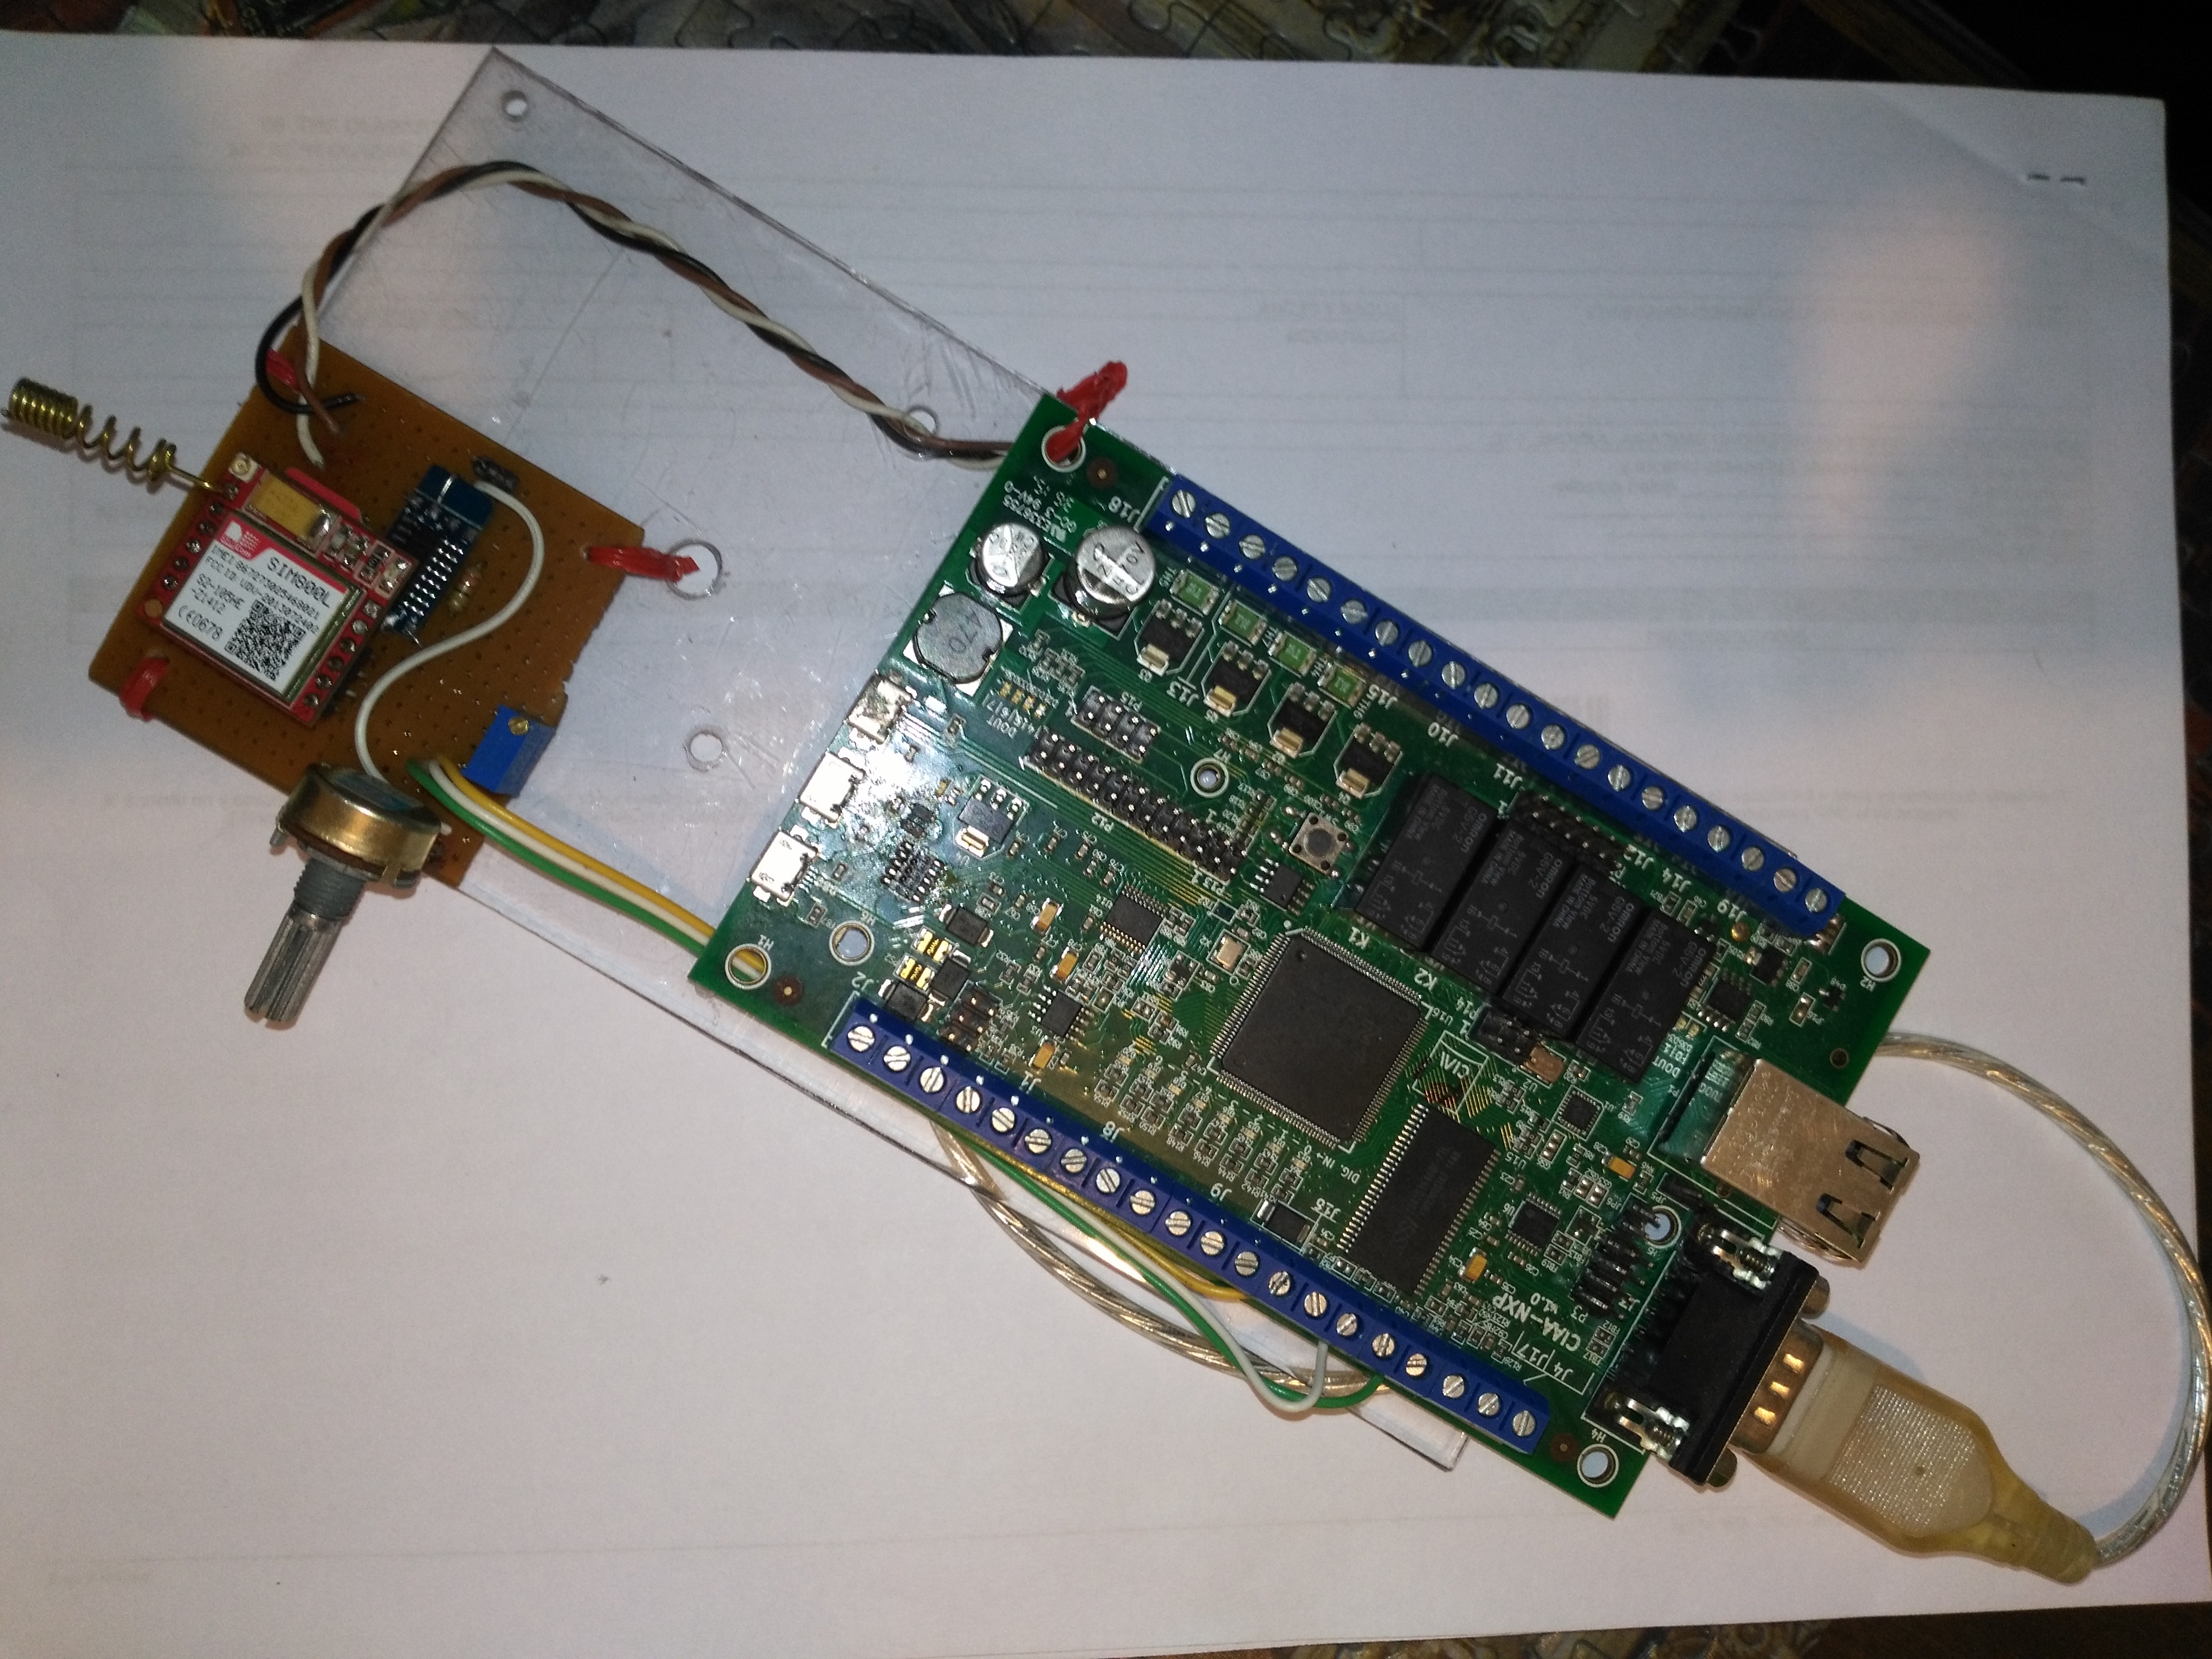
\includegraphics[scale=.1]{./Figures/prototipo.jpg}
  \caption{Placa básica integrada con la CIAA-NXP.}
  \label{fig:prototipo}
\end{figure}

\section{Configuraciones para la PC}

Para la realización de los ensayos, se configuró la PC en forma adecuada. En la figura \ref{fig:hw_pc} se puede ver cómo configurar en Linux la interfaz de red. Es importante destacar que dichos comandos son ejecutados con el permiso de usuario \emph{root}.

\begin{figure}[h]
  \centering
  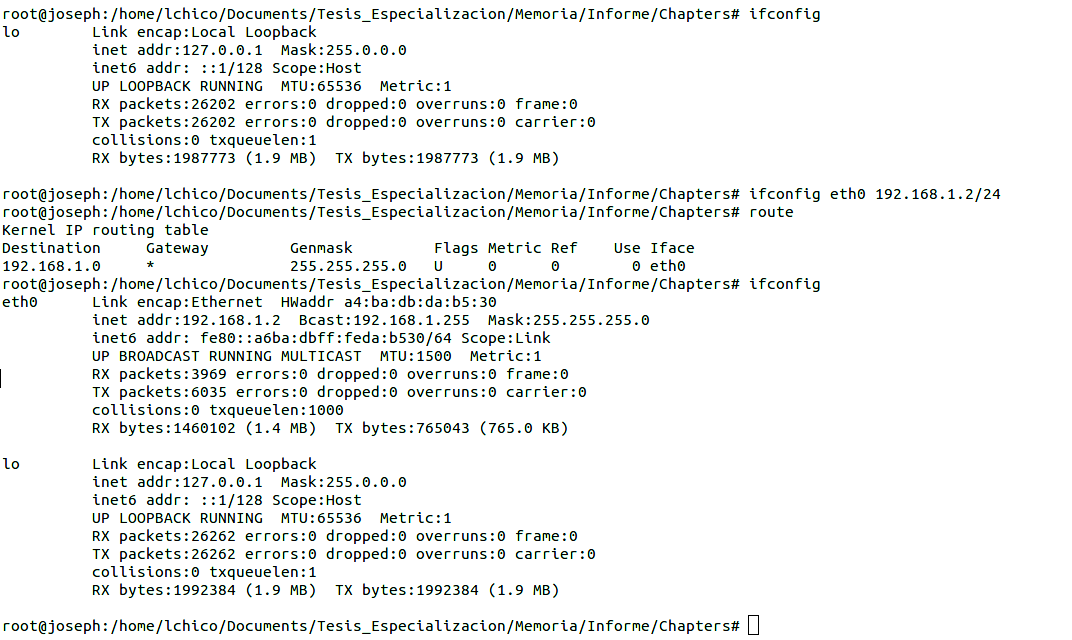
\includegraphics[scale=.45]{./Figures/config_net_console.png}
  \caption{Configuración de una red estática para la interfaz Ethernet.}
  \label{fig:hw_pc}
\end{figure}

Una vez que se tiene la configuración de red adecuada se obtiene en el navegador web la imagen \ref{fig:web_monitoreo} que fue introducida en el capítulo 3.

\begin{figure}[h]
  \centering
  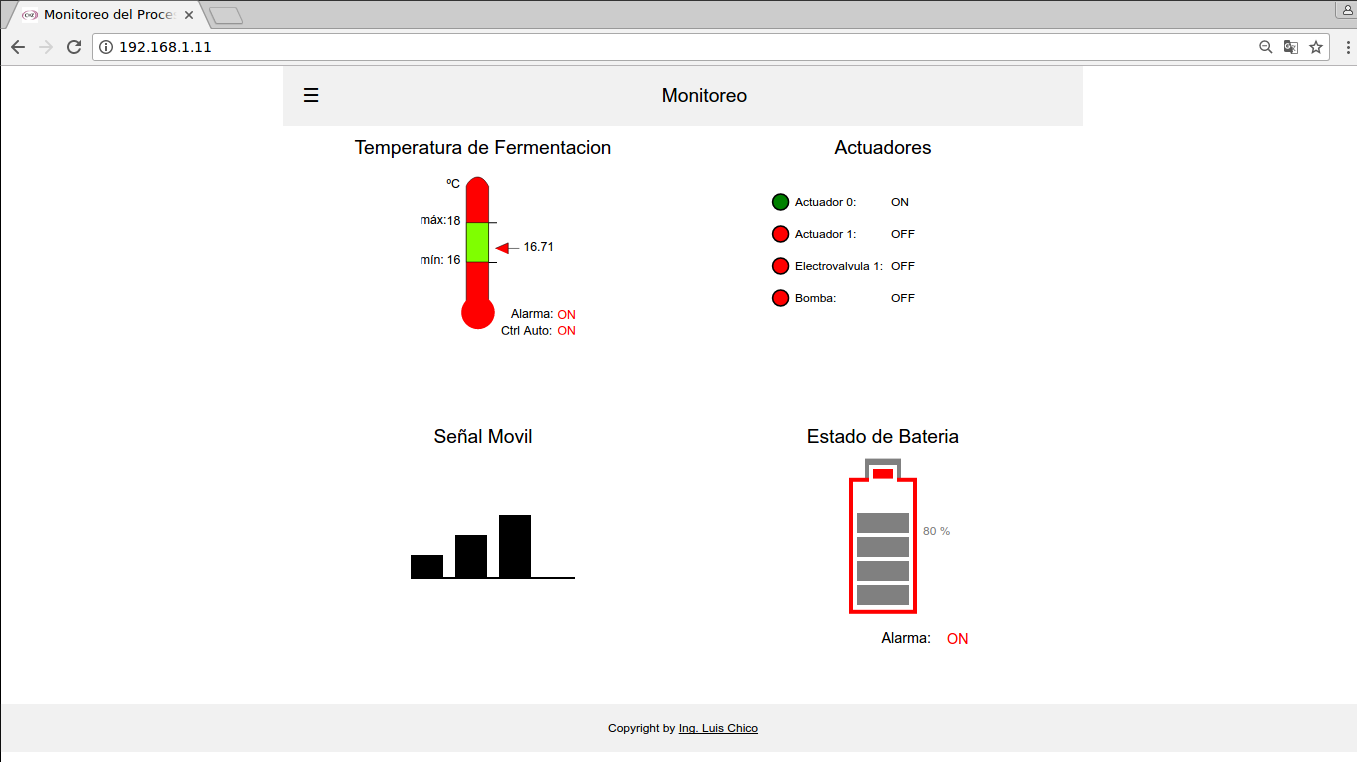
\includegraphics[scale=.25]{./Figures/web_monitoreo.png}
  \caption{Pantalla principal de la web de monitoreo.}
  \label{fig:web_monitoreo}
\end{figure}

En esta pantalla se tiene toda la información correspondiente al sistema. 
Arriba a la izquierda se ve el estado de la temperatura, con sus rangos máximos y mínimos seteados. Y debajo de dicho termómetro podemos ver si esta activada: la alarma y el control automático.

Luego arriba y a la derecha los estados de los actuadores, la electroválvula y la bomba. Estos le permiten al cliente controlar en forma remota dos actuadores y el sistema correspondiente a la bomba de refrigeración con la electroválvula asociada. El sensor de temperatura permitirá informarle al sistema de control automático cuando debe actuar acorde a los rangos establecidos, esto solo en el caso de estar activado dicho control automático. 

Abajo a la izquierda el nivel de señal correspondiente al módem GSM, mediante el cual podremos saber si la cobertura de señal de la red de telefonía móvil esta en condiciones de operar y entonces estaría disponible el servicio de alertas mediante mensajes SMS. 

Finalmente abajo a la derecha el estado de la batería, el cual va a permitir al sistema continuar en funcionamiento en caso de un corte de energía. El principal uso de este será mantener la posibilidad de enviar un mensaje SMS notificando el corte de energía.


%----------------------------------------------------------------------------------------
%	SECTION 1
%----------------------------------------------------------------------------------------

\section{Pruebas funcionales del hardware}
\label{sec:pruebasHW}

Una vez recorrido todas las opciones que permite la interfaz web y verificar que el comportamiento haya sido el esperado. Se procede interactuar con el sistema, por medio de alteraciones generadas a través de los potenciómetros que representaran la temperatura y el estado de la batería.

Estando activado el control automático y al simular un incremento de temperatura, se comprobó que al exceder la temperatura máxima inicio en forma automática la bomba que permite la circulación del refrigerante y la activación de la electroválvula que interviene sobre el tanque que se está monitoreando. En el navegador web se verá como en la figura \ref{fig:auto_control_active}. y en la figura \ref{fig:sms_min_max_bat} se puede observar la alerta correspondiente mediante un SMS.

\begin{figure}[h]
  \centering
  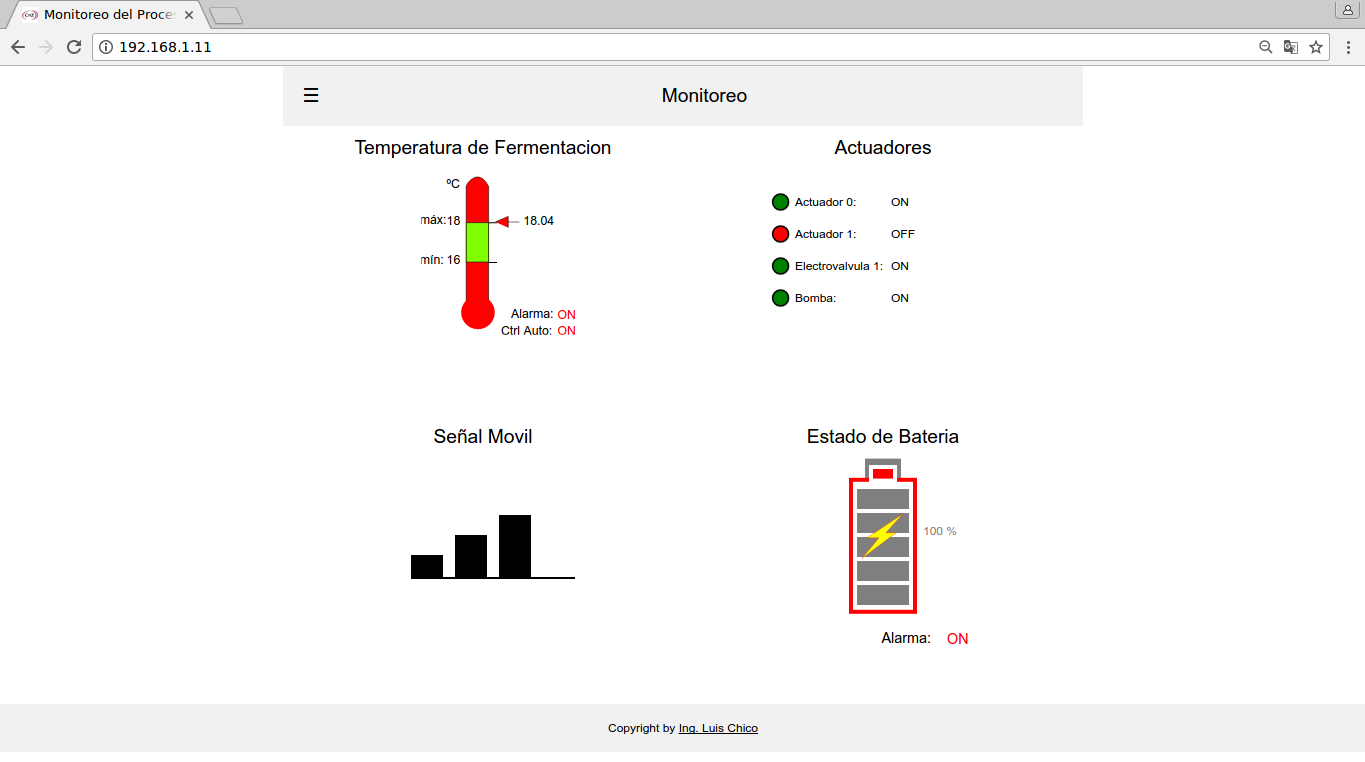
\includegraphics[scale=.25]{./Figures/auto_control_active.png}
  \caption{Activación por control automático debido a temperatura elevada.}
  \label{fig:auto_control_active}
\end{figure}


\begin{figure}[h]
  \centering
  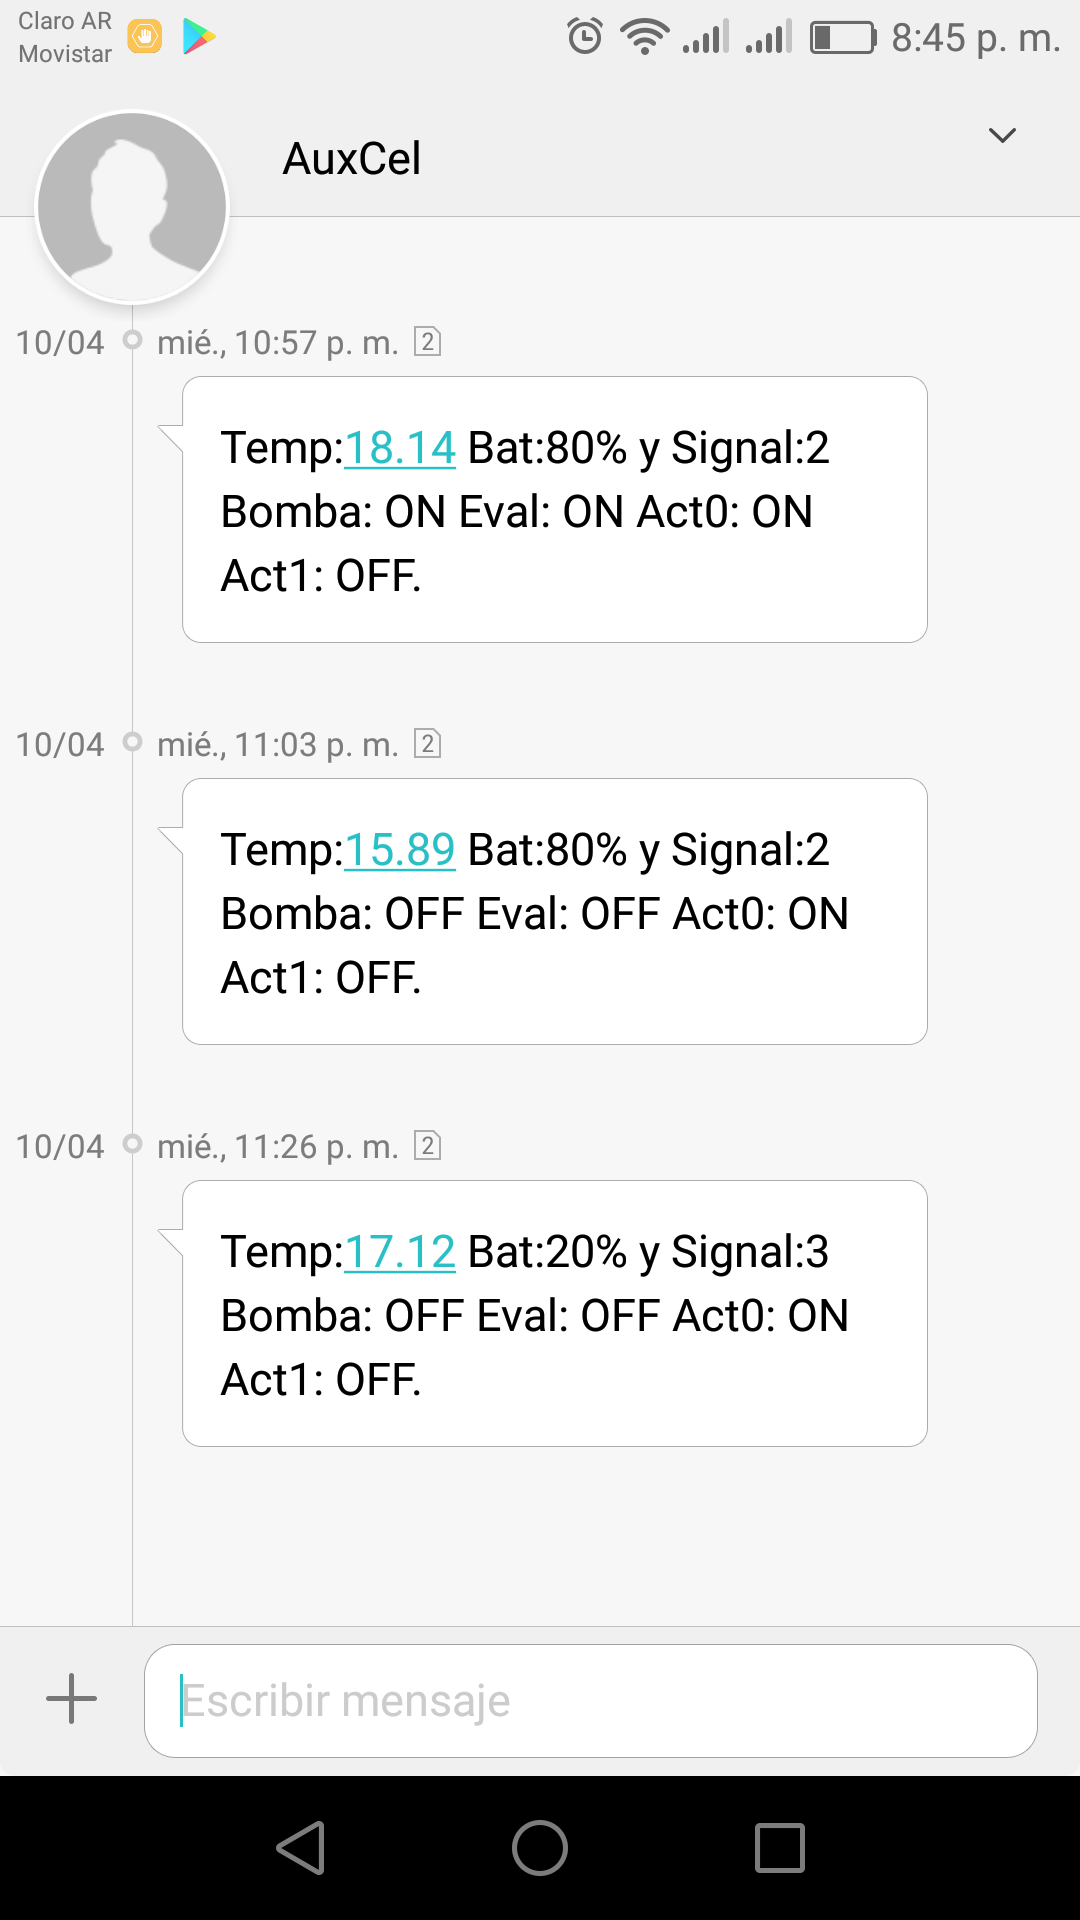
\includegraphics[scale=.15]{./Figures/sms_min_max_bat.png}
  \caption{SMS recibidos debido a temperatura máxima. \\
   El segundo SMS recibido es por temperatura mínima. \\
   Y el último recibido debido a batería baja.}
  \label{fig:sms_min_max_bat}
\end{figure}

Se verificó que el estado de la bomba y la electroválvula se mantiene activado hasta llegar a la temperatura mínima, en este instante se procede a desconectar la bomba y a cerrar la electroválvula. En la web se mostrará  como en la figura \ref{fig:auto_control_inactive}. y dado su respectiva alerta mediante un SMS como en la figura \ref{fig:sms_min_max_bat}

\begin{figure}[h]
  \centering
  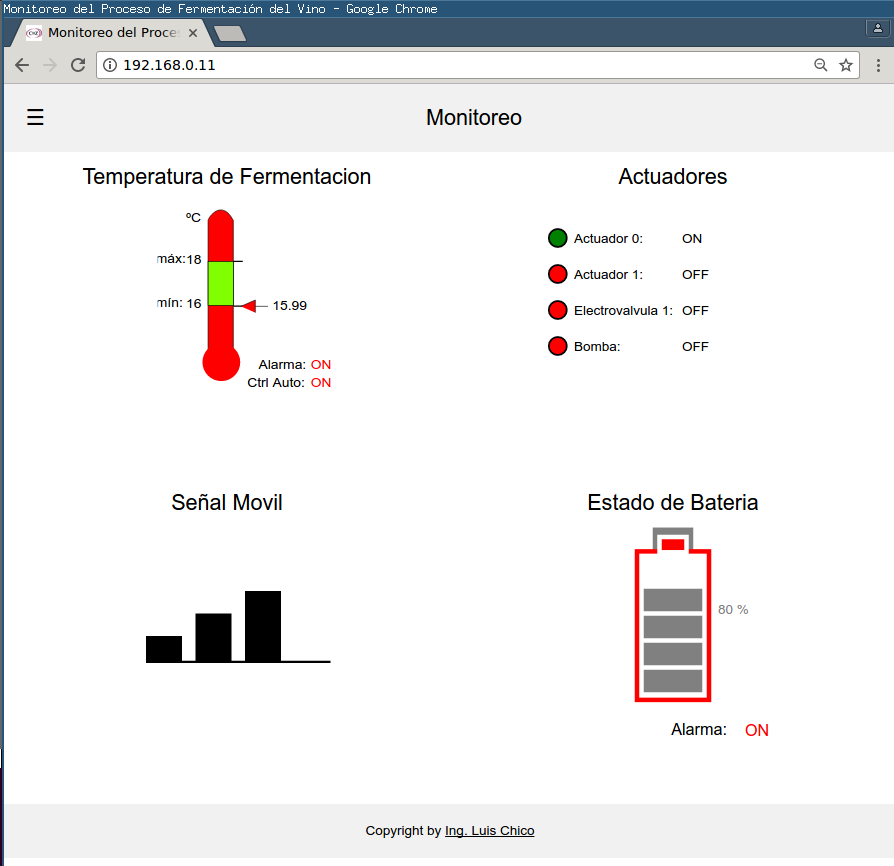
\includegraphics[scale=.3]{./Figures/auto_control_inactive.png}
  \caption{Temperatura en nivel mínimo, se desactiva la bomba y la electroválvula.}
  \label{fig:auto_control_inactive}
\end{figure}


En el caso de la batería se analiza las variaciones en la carga.
Si esta disminuye más de un valor que es determinado, se envía un SMS como en la figura \ref{fig:sms_min_max_bat}. 
Es importante aclarar que en caso de producirse un corte de energía, el sistema no está pensado para que se mantenga en funcionamiento por un tiempo prolongado, sino más bien lo que se busca es que este pueda mantener informado a la personas responsables que se requiere de su atención. 
Es por esto que no se realizó un estudio del tiempo de vida del sistema.

Para verificar los actuadores, se tiene la sección de configuración de actuadores y para cada uno de ellos se verificó los diferentes estados, encendiendo y apagando. Luego se probó en bloques de varios actuadores. En la figura \ref{fig:test_contact} se ve un ejemplo de los casos probados.

\begin{figure}[h]
  \centering
  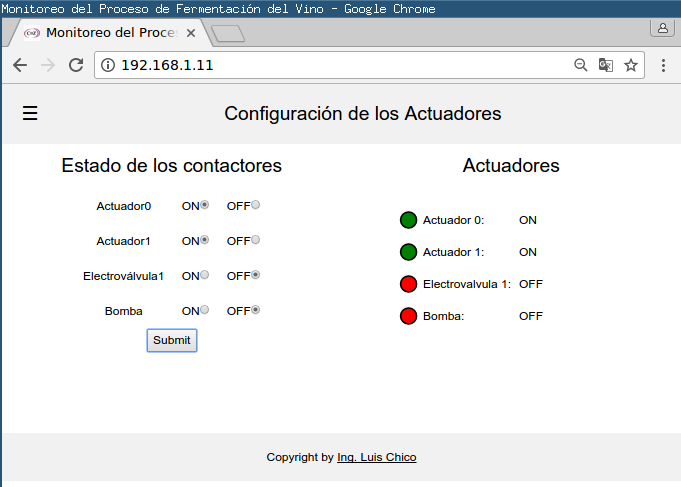
\includegraphics[width=1\linewidth]{./Figures/test_contact.png}
  \caption{Activación manual de actuador 1 y 2, electroválvula y bomba inactivo.}
  \label{fig:test_contact}
\end{figure}


De esta forma concluyó que el funcionamiento del sistema es el correcto.


